\setAuthor{Sandra Schumann}
\setRound{piirkonnavoor}
\setYear{2023}
\setNumber{G 5}
\setDifficulty{5}
\setTopic{TODO}

\prob{Vedru keerutamine}
\begin{wrapfigure}{r}{0.3\textwidth}
  \vspace{-2em}
  \begin{center}
    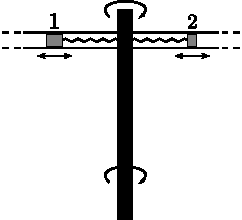
\includegraphics[width=1\linewidth]{2023-v2g-05-yl.pdf}
  \end{center}
  \vspace{-2em}
\end{wrapfigure}

Kaks erineva jäikusega, kuid sama pikkusega vedru on kinnitatud ühest otsast posti külge. Kummagi vedru teises otsas on raskus, kusjuures esimese vedru otsas olev raskus on kaks korda suurema massiga kui teise vedru otsas olev raskus. Mõlemad vedrud asuvad hõõrdevabas kanalis, kus raskused saavad liikuda ainult horisontaalselt, mistõttu gravitatsiooniga arvestama ei pea. Post hakkab pöörlema nii, et ka vedrude otsas olevad massid hakkavad liikuma ringsel trajektooril. Selle peale pikeneb esimene vedru kaks korda ja teine neli korda. Mis on vedrude jäikuste suhe? Vedrude enda massid võib lugeda raskuse massiga võrreldes tühiselt väikeseks. Eeldage, et vedru pikenemine on piisavalt väike selleks, et kehtiks Hooke'i seadus.


\hint

\solu
Olgu vedrude jäikused $k_1$ ja $k_2$, raskuste massid vastavalt $2m$ ja $m$, posti nurkkiirus $\omega$ ning vedrude algne pikkus $l$. Siis pikeneb esimene vedru pikkuse $2l - l = l$ võrra ja teine $4l - l = 3l$ võrra \p{1}. Esimese vedru pikenemisest tulenev jõud on $k_1 \cdot l$ ja teise vedru pikenemist tulenev jõud on $k_2 \cdot 3l$ \p{2}. Ringliikumisest saame ka, et esimese jõu suurus peab olema $2m \omega^2 \cdot 2l$ ja teise jõu suurus $m \omega^2 \cdot 4l$ \p{2}. Saame kirja panna, et:

$$k_1 \cdot l = 2m \omega^2 \cdot 2l$$
$$k_2 \cdot 3l = m \omega^2 \cdot 4l$$
$$\frac{k_1}{k_2} = \frac{2m \omega^2 \cdot 2l}{m \omega^2 \cdot 4l} \cdot \frac{3l}{l} = \frac{2 \cdot 2 \cdot 3}{4 \cdot 1} = 3$$

Vedrude jäikuste suhe on 3-kordne \p{3}.
\probend